\documentclass[10pt]{article}
\setlength{\parskip}{0.25\baselineskip}
\usepackage[margin=1in]{geometry} 
\usepackage{amsmath,amsthm,amssymb, graphicx, multicol, array}
\usepackage[font=small,labelfont=bf]{caption}
\usepackage{tikz}
\usepackage{float}

\newcommand{\supp}{{\text{supp}}} 
\newcommand{\bv}{{\text{BV}}}
\newcommand{\ac}{{\text{AC}}}

\newenvironment{problem}[2][]{\begin{trivlist}
\item[\hskip \labelsep {\bfseries #1}\hskip \labelsep {\bfseries #2.}]}{\end{trivlist}}

\begin{document}
 
\title{Homework \#4}
\author{Eric Tao\\
Math 233: Homework \#4}
\maketitle

\begin{problem}{Question 1}

Let $L_1, L_2$ be lines in the plane. For which pairs of $L_1, L_2$ do there exists real functions, harmonic on the entire plane, 0 on $L_1 \cup L_2$, but not vanishing identically?

\end{problem}
\begin{proof}[Solution]

First, we notice that for any real function $v$, harmonic on the entire plane, it is the imaginary part of some holomorphic function. First, we know already that by 11.10, every real harmonic function is the real part of a holomorphic function, locally at least. Then, by considering disks around every point $z \in \mathbb{C}$, this can be extended to a holomorphic function $f$ such that $\Re(f) = v$, because on the disks, the local holomorphic functions may only differ by an imaginary constant, and it must align on intersections of disks, thus there may only be a single entire function.

Now, consider $i f$. Since $i$ is a constant, this is clearly holomorphic. Further, by construction $\Im(f) = v$. Thus, we have a holomorphic function such that $v$ is its imaginary part.

Now, suppose $v$ is harmonic, and $v(L_1) = 0, v(L_2) = 0$. Without loss of generality, since we may translate $v$ without affecting the derivatives, we may take $L_1 \cap L_2 = \{ (0,0)\}$. By a further linear change of coordinates, we may assume that $L_1$ is the real line, which will keep $v_{xx} + v_{yy} = 0$. 

Suppose $L_1$ and $L_2$ intersect.  Suppose that the angle between $L_1, L_2$ is $\theta_0$.

By the Schwarz reflection principle (11.14), and a relabeling of the two lines as need be, if we call $\sigma_1, \sigma_2$ the reflections of the plane with respect to $L_1, L_2$, we must have that $f(\sigma_1(z)) = \overline{f}(z), f(\sigma_2(z)) = \overline{f}(z)$. In particular then, on $L_1, L_2$, we have that $v(\sigma_1(z)) = v(z) = 0, v(\sigma_2(z)) = v(z) = 0$. Pictorially:

\begin{figure}[H]
\centering
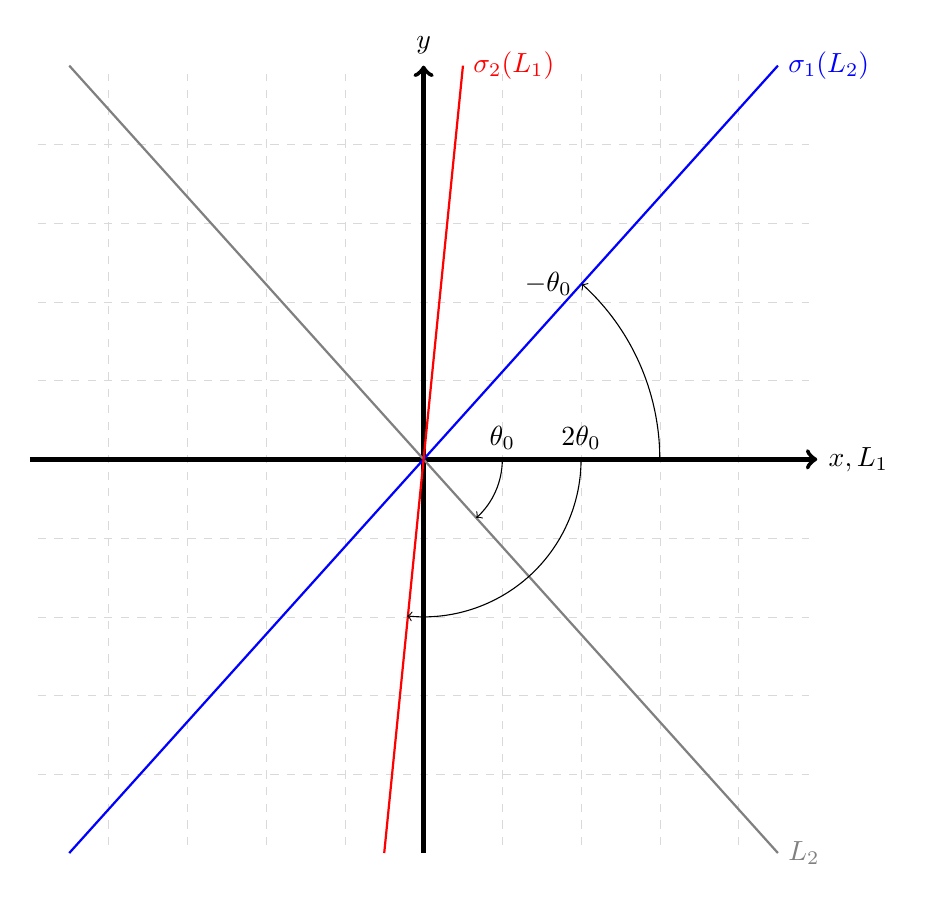
\begin{tikzpicture}
\draw[help lines, color=gray!30, dashed] (-4.9,-4.9) grid (4.9,4.9);
\draw[->,ultra thick] (-5,0)--(5,0) node[right]{$x, L_1$};
\draw[->,ultra thick] (0,-5)--(0,5) node[above]{$y$};
\draw[gray, thick] (-4.5,5) -- (4.5,-5) node[right]{$L_2$};
\draw[blue, thick] (-4.5, -5) -- (4.5, 5) node[right]{$\sigma_1(L_2)$};
\draw[red, thick] (-0.5, -5) -- (0.5, 5) node[right]{$\sigma_2(L_1)$};
\draw[black, ->] (1,0) node[above]{$\theta_0$} arc (0:-48:1) ;
\draw[black, ->] (2,0)  node[above]{$2\theta_0$} arc (0:-96:2);
\draw[black, ->] (3,0) arc (0:48:3)  node[left]{$-\theta_0$} ;
\end{tikzpicture}
\end{figure}

where we have that the angle between $L_1, \sigma_1(L_1)$ is $2 \theta_0$ because the angle between $\sigma_1(L_1)$ and $L_2$ is $\theta_0$, due to how reflections work. Further, we also see that $\sigma_1(L_2)$ takes on the angle $- \theta_0$.

We notice that we may iterate this process, and in fact generate lines of $k\theta_0$ via successive reflections. However, we know that if $\theta_0$ is not a rational multiple of $\pi$, then $\{ e^{im\theta_0} :m \in \mathbb{Z} \}$ is dense in $T$. And since $v = 0 $ on all of these lines, if it is $0$ on a dense set, then it is $0$ everywhere by continuity. Thus, this implies that we must have that $\theta_0$ is a rational multiple of $\pi$.

Now, suppose instead that $L_1, L_2$ are parallel. In such a case, applying the Schwarz reflection principle on successive lines, we note that then we must have that $v$ is periodic, $0$ at each interval $d = \text{dist}(L_1, L_2)$, since we can keep translating and applying reflections to find a line on the opposite side. For example, assuming $L_1: x = 1, L_2: x = 5$ one such $v$ could be $v(x,y) = e^{y} \sin(\pi(x-1)/\pi)$. This is generalizable with a suitable linear transformation on $x,y$ to match our parallel 1-D lattice.

\end{proof}

\begin{problem}{Question 2}

Suppose $\Delta$ is a closed equilateral triangle in the plane, with vertices $a,b,c$. Find $\max\{ |z-a||z-b||z-c| \}$ for $z \in \Delta$. 

\end{problem}

\begin{proof}[Solution]

First, fix some $a,b,c \in \mathbb{C}$. We notice that the function:

$$ f(z) = (z - a)(z-b)(z-c)$$ 

is a polynomial, thus entire. Then, we may apply the maximum modulus principle to our closed triangle which then says that:

$$ |z-a||z-b||z-c| \leq \Vert (z-a)(z-b)(z-c) \Vert_{\partial \Delta} $$

Thus, it is sufficient to consider the value of $(z-a)(z-b)(z-c)$ on the boundary of our equilateral triangle. Further, since the quantity we are concerned about is

$$\Vert (z-a)(z-b)(z-c) \Vert_{\partial \Delta} = \max\{ |z-a||z-b||z-c| : z \in \partial \Delta \} $$

where we use max instead of sup due to being compact, this is simply the product of the distances from $z$ to $a,b,c$. Thus, under any isometries, this product is preserved. Therefore, we may take rotations and translations such that the following picture holds, for $2s$ the side length of our triangle:

\begin{figure}[H]
\centering
\begin{tikzpicture}
\draw[->,ultra thick] (-5,0) -- (5,0);
\draw[->,ultra thick] (0,-5) -- (0,5);
\draw[red, thick] (-1,0) node[below left]{$(-s,0)$} -- (1,0) node[below right]{$(s,0)$};
\draw[red, thick] (-1,0) -- (0,1.73) node[right]{$(0,\sqrt{3}s)$};
\draw[red, thick] (1,0) -- (0,1.73);
\end{tikzpicture}
\end{figure}

Due to symmetries, we can also restrict ourselves to analyzing $z$ on the real line, as a simple rotation will find us the value on the other sides. It should also be clear that due to reflectional symmetries, we can restrict ourselves to the non-negative reals as well.

Let $z = (x,0)$ with $x \in [0,s]$. Computing the value of $|f|$, we find:

$$|f(z)| = |(x,0) - (s,0)| + |(x,0) - (-s,0)| + | (x,0) - (0,\sqrt{3} s)| = (s- x)(x + s)\sqrt{x^2 + 3s^2} = (s^2 - x^2)\sqrt{x^2 + 3s^2} $$

But now, this is a real function, so we may take a derivative and check endpoints to find the maximum. We see pretty clearly that:

$$ f’(x) = -2x\sqrt{x^2 + 3s^2} + x(s^2 - x^2)\frac{1}{ \sqrt{x^2 + 3s^2} } = \frac{1}{ \sqrt{x^2 + 3s^2} } \left(-2x(x^2 + 3s^2) + x(s^2 - x^2) \right) =  $$

$$ \frac{1}{ \sqrt{x^2 + 3s^2} } (-3x^3 - 5xs^2) = \frac{1}{ \sqrt{x^2 + 3s^2} } x(-3x^2-5s^2)$$

Clearly, since $x^2 \geq 0, s^2 > 0$, we have that $x^2 + 3s^2$ and $-3x^2-5s^2$ never vanish. Thus, we have only the critical point $x = 0$. Since at $x=s$, $f$ vanishes, because this is also a boundary of our domain, this must be the maximum. Thus, we have that the maximum of $f$ is equal to:

$$ f(0) = s^2 \sqrt{3s^2} = \sqrt{3} s^3$$ where $2s = |a - b | = |b - c| = |c - a|$

\end{proof}

\begin{problem}{Question 3}

Suppose $f \in \mathcal{H}(\Pi^+)$, where $\Pi^+= \{ z = x + yi : y > 0 \}$, and $|f| \leq 1$. How large can $|f'(i)|$ be? Find the extremal functions.

\end{problem}

\begin{proof}[Solution]

First, for $U = \{ z : |z| < 1 \}$, we consider the map $\psi: U \to \Pi^+$ via:

$$\psi(z) = i \frac{1 - z}{1 + z} $$.

On $U$, this map is holomorphic. Further, this is injective. Suppose we have that $\psi(z) = \psi(w)$. Then, since on $U$, $z, w \not = -1$:

$$ i \frac{1 - z}{1 + z} = i\frac{1 - w}{1 + w} \implies (1 + w)(1 - z) = (1+ z)(1-w) \implies 1 + w - z - wz = 1 + z - w - wz \implies 2w = 2z \implies w = z$$

Further, we have that this map is surjective onto $\Pi^+$. Let $\zeta = a + bi \in \Pi^+$. Then, we have that, for $z = x + yi$:

$$ f(z) = \zeta \iff i \frac{1 - x - yi}{1 + x + yi} = a + bi \iff 1 - x - yi = -ai - axi + ay + b + bx + byi $$
$$ \iff \begin{cases} 1 - x = ay + b + bx \\ -y = -a - ax + by\end{cases} \iff x = \frac{1 - ay - b}{1 + b}$$

where we've used the fact that $z \in U$ so $1 + x + yi \not = 0$ and $\zeta = \Pi^+$, so $b \not = -1$. Now, substituting into the second equation, this would enforce that:

$$ -y = -a - a\frac{1 - ay - b}{1 + b} + by \iff -y\left(1 + b + \frac{a^2}{b+1}\right) = -a- \frac{a - ab}{1 + b} = \frac{-2a}{1 + b} \iff$$

$$ y = \frac{2a}{1 + b} \cdot \frac{b+1}{ a^2 + (b+1)^2} = \frac{2a}{a^2 + (b+1)^2} $$

Now, substituting back in for $x$, we find that:

$$ x  =  \frac{1 - a  \frac{2a}{a^2 + (b+1)^2} - b}{1 + b} = \frac{1}{1 + b} \cdot \frac{a^2 + (b+1)^2 - 2a^2 - a^2b - b(b+1)^2}{a^2 + (b+1)^2} = \frac{1}{b+1} \frac{-a^2(b+1) + (b+1)^2(1-b)}{a^2 + (b+1)^2}=$$
$$ \frac{ 1 - a^2 - b^2}{a^2 + (b+1)^2} $$

Now, we need only check that this lives within $U$. Well:

$$ x^2 + y^2 = \frac{1}{(a^2 + (b+1)^2)^2} [ (1 - a^2 - b^2)^2 + 4a^2] $$

It should be clear that this is always less than the denominator. If we expand everyyhing out, we see that we have the numerator as:

$$ 1 + a^4 + b^4 + 2a^2 - 2b^2 + 2a^2b^2 $$

and the denominator as:

$$ a^4 + 2a^2(b+1)^2 + (b+1)^4 = a^4 + 2a^2b^2 + 4a^2b + 2a^2 + b^4 + 4b^3 + 8b^2 + 4b + 1 $$

Subtracting the numerator from the denominator, we see:

$$ (a^4 + 2a^2b^2 + 4a^2b + 2a^2 + b^4 + 4b^3 + 8b^2 + 4b + 1) -  (1 + a^4 + b^4 + 2a^2 - 2b^2 + 2a^2b^2) = $$
$$ 4a^2b+ 4b^3+ 10 b^2 + 4b $$

Now, because $(a,b)$ are chosen from the upper half plane, we have that this number must be positive, since $a^2 \geq 0$, and $b > 0$. Thus, we have that $x^2 + y^2 < 1$, and therefore $z \in U$. Thus, $\psi$ is surjective.

Lastly, we consider the action of $\psi$ on $T = \{ z : |z| = 1 \}$, or really, $T \setminus \{ -1 \}$. Well, if $|z| = 1$, we may write it as $z = e^{i \varphi}$. First, we notice that:

$$\begin{cases} \sin(x) = \frac{e^{ix} - e^{-ix}}{2i} \\ \cos(x) = \frac{e^{ix} + e^{-ix}}{2} \end{cases} \implies \tan(x) = i \frac{e^{ix} - e^{-ix}}{e^{ix} + e^{-ix}} = i \frac{e^{2ix} - 1}{e^{2ix} + 1}$$

Then, we have that:

$$ \psi(e^{i\varphi}) = i \frac{1 - e^{i\varphi}}{1 + e^{i\varphi}} = -i \frac{ e^{i\varphi} - 1}{1 + e^{i\varphi}} = -i \cdot i \tan\left(\frac{\varphi}{2}\right) =  \tan\left(\frac{\varphi}{2}\right)$$

Since on $T \setminus \{ -1 \}$, $\varphi \in (-\pi, \pi)$, and on $x \in (-\pi/2, \pi/2)$, $\tan(x) \in (-\infty, \infty)$, $\tan(\varphi/2)$ covers the real line.

Now, let $f$ be as given, and consider the map $g = f \circ \psi: U \to \mathbb{C}$. Because $|f| \leq 1$ on the upper half plane, and the work we've done above, we have that $g \in \mathcal{H}^\infty(U)$, $\Vert g \Vert_\infty \leq 1$, and since $g$ is defined on $U$, we have that, as stated in 12.5, we may take $\alpha = 0 < 1$. Further, if $g(0) = \beta$, then we may assume that $| \beta | < 1$, as otherwise, by the maximum modulus principle, since $|g| \leq 1$ on $U$, this extends to the boundary by continuity. So, if $|g(0)| = 1$, then $g$ is constant everywhere and the derivative is 0.

Then, by the discussion in 12.5, we have that:

$$ |g'(0)| \leq 1 - | \beta |^2 $$

However, here, we notice that because $g = f \circ \psi$, $\psi(0) = i \frac{ 1 - 0}{ 1+ 0} = i$, so $g'(0) = f'(i), g(0) = \beta = f(i)$. 

Thus, restated in terms of $f$, we have that:

$$ |f'(i)| \leq 1 - | f(i)|^2 $$

Thus, we have two conditions to realize the maximum value here across all functions $f$. Firstly, we require $f(i) = 0$, and secondly, by Theorem 12.2, if $f(i)= \beta = 0$, then we have that $|g'(0)|  = 1$ occurs if and only if $g = \lambda z$, for some $\lambda \in \mathbb{C} : | \lambda | = 1$, that is, $f$ composed with $\psi$ acts as a rotation by some $\lambda$ on the unit disk $U$. 

This means that, we need only take an inverse to $\psi$, with some scale factor for the rotation, and a translation such that $f(i) = 0$. Well, I claim that $f(z) = \frac{iz + 1}{-iz + 1}$ acts as a left inverse to $\psi$:

$$ f\left(i \frac{1-z}{1+z}\right) = \frac{- \frac{1-z}{1+z} + 1}{ \frac{1-z}{1+z} +1} = \frac{ -1 + z + z + 1}{ 1-z + 1 + z} = \frac{2z}{2} = z$$

Further, we see that $f(i) = \frac{i^2 + 1}{-i^2 + 1} = \frac{0}{2} = 0$. So that part is all set.

Then, the maximal functions take on exactly the form $f_\lambda(z) = \lambda  \frac{iz + 1}{-iz + 1}$ for $\lambda \in \mathbb{C} : |\lambda| = 1$. 

\end{proof}

\begin{problem}{Question 4}

Suppose $f \in \mathcal{H}(\Omega)$. Under what conditions can $|f|$ have a local minimum in $\Omega$?

\end{problem}
 
\begin{proof}[Solution]

We see that for $f$ non-constant, $|f|$ may have a local minimum on a  connected component of $\Omega$ if and only if $f$ never attain 0 on that component. Equivalently, we prove that $|f|$ has a non-0 local minimum on a connected component if and only if $f$ is constant on that component.

For what follows, let $\Omega$ be a single connected component. Clearly, if $f$ is a non-0 constant, then $|f|$ has a non-0 local minimum, as at any point $\zeta \in \Omega$, $f(\zeta) = f(z) \implies f(\zeta) = f(z)$ for all $z \in \Omega$. So we need only prove the other direction.

Suppose $|f|$ has a non-0 local minimum at $\zeta \in \Omega$, that is, $0 < |f(\zeta)| \leq |f(z)|$ for all $z \in \Omega$. Then, $f$ has no 0s on $\Omega$, but is holomorphic. Thus, $g = 1/f$ is a holomorphic function on $\Omega$. In particular, at $\zeta$ we have that $ g(\zeta) = \frac{1}{f(\zeta)}$. Since $|f|$ is at a minimum at $\zeta$, $|g| = |1/f|$ is at a maximum at $\zeta$. Thus, we would have that $|g|$ has a local maximum on $\Omega$. However, by the maximum modulus principle, since $|g|$ has a local maximum, we have that $g$ is constant. But, if $g$ is constant, then since $g = 1/f \implies f = 1/g$, $f$ too must be constant.

Thus, $|f|$ having a positive local minimum is equivalent to $f$ being constant on the component containing a local minimum.

\end{proof}
  

\begin{problem}{Question 5}

(a) Suppose that $\Omega$ is a region, $D$ is a disc, $\overline{D} \subset \Omega$,$f \in \mathcal{H}(\Omega)$, non-constant, and $|f|$ is constant on $\partial D$. Prove that $f$ has at least one zero in $D$. 

(b) Find all entire functions $f$ such that $|f(z)|  =1 $ for all $|z| = 1$. 

\end{problem}

\begin{proof}[Solution]

(a)

Since $\overline{D}$ is compact and $|f|$ is a continuous function, $|f|$ achieves a minimum somewhere on $\overline{D}$. First, suppose $|f| \geq \delta > 0$ on $\overline{D}$.

If this occurs on the interior, then by the last problem, $f$ must be constant on $D$, a contradiction. Thus, suppose this occurs on the boundary, that is $|f|$ attains a minimum on $\overline{D}$ on $\partial D$. Since $|f|$ is constant, the minimum is attained at all points on the boundary, call it $a$. However, by the maximum modulus principle, we have that $|f(z)| \leq \Vert f \Vert_{\partial D} = a$ for all $z \in D$. Thus, we have that for all $z \in D$, $a = \Vert f \Vert_{\partial D} \leq |f(z)| \leq \Vert f \Vert_{\partial D} = a \implies |f(z)| = a$. Since $f$ is holomorphic, for this to satisfy the Cauchy-Riemann equations on a disk, we must have that $f$ is constant. Thus, we cannot have that we achieve a positive minimum anywhere.

Now, suppose that $|f|$ achieves 0 somewhere. If it is on the boundary, because $|f|$ is constant on the boundary, then $|f| = 0$ on all of $\partial D$. However, by the maximum modulus principle then, $f = 0$ everywhere, a contradiction. Then, we must have that $|f| = 0$ somewhere on $D$, and thus $f = 0$ somewhere on $D$.

(b)

We claim that under these hypotheses, this is satisfied only if $f = cz^m$ for some $m \geq 0$ and $c \in \mathbb{C}$ such that $|c| = 1$. Clearly, if $f$ is constant, then any function that satisfies this is just $f = e^{i \theta}$ for $\theta \in [0,2\pi)$ and this satisfies the above conditions for $m = 0$. 

So, assume $f$ is non-constant. Let $m$ be the multiplicity of the zero of $f$ at $z = 0$, with $m = 0$ if $f(0) \not = 0$. Define:

$$f_1(z) = \frac{f(z)}{z^m}$$

We notice the following. When $|z| = 1$, we have that $|f_1(z)| = \frac{|f(z)|}{|z|^m} = \frac{1}{1} = 1$, and that by definition, for $m \not = 0$, we can find a $h(z)$ such that $f(z) = z^m h(z)$ on $\Omega$ with $h(0) \not = 0$, that

$$f_1(z) = \frac{f(z)}{z^m} = \frac{z^m h(z)}{z^m} = h(z)$$

and thus $f_1(0) \not = 0$.

Now, if $f_1(z)$ is constant, we are done, since of course, we must have that $|\lambda| = 1$, as:

$$f_1(z) = \lambda \implies \frac{f(z)}{z^m} = \lambda \implies f(z) = \lambda z^m$$

and since by hypothesis, when $|z| = 1$, $|f(z)| = 1$, therefore $|\lambda| = 1$.

Then, suppose $f_1(z)$ is not constant. Then, by part (a), we must have at least one zero on $U$, away from $z= 0$. Let $\alpha_1,...,\alpha_m$ be the zeros of $f_1$ in $U$ with multiplicity according to the order of the zero.Recall the function defined in Rudin (12.4) as:

$$\varphi_\alpha(z) = \frac{z - \alpha}{1 - \overline{\alpha}z} $$

Then, consider the function:

$$g(z) = \frac{f_1(z)}{\varphi_{\alpha_1}(z) ... \varphi_{\alpha_m}(z)} = f_1(z) \cdot \prod_{j=i}^m \frac{1 - \overline{\alpha}_j z}{z - \alpha_j}$$

We notice that by construction, $g$ must be holomorphic on $U$, because suppose $f_1$ has a zero of order $m$ at $\alpha_i$. Then we may write $f_1 = (z-\alpha_i)^m h(z)$ for some holomorphic function $h_{\alpha_i}$ that is non-0 at $\alpha_i$. Further, by construction, since we counted $\alpha_i$ as zeros of $f$ with multiplicity according to the order of the 0, there are exactly $m$ copies of $\frac{1}{z-\alpha_i}$ in the product. Thus, $g$ has a removable singularity at each 0 of $f_1(z)$.

Further, suppose $g = 0$ on $U$. This cannot happen at any of the zeros of $f_1$, due to the analysis presented above, as the order of the zero is cancelled out by the denominators, and we are left with a non-0 function, as $(1 - \overline{\alpha_j}\alpha_i) = 0 \iff  \overline{\alpha_j}\alpha_i = 1$, which implies that $| \overline{\alpha_j} | = | \alpha_j | = \frac{1}{|\alpha_i} > 1$. But since $\alpha_j$ is a 0 of $f_1$ in $U$, $|\alpha_j| < 1$, so this cannot happen. Further, by the same logic, none of the $1 - \overline{\alpha_j} z$ disappear on $U$. Thus, $g$ is non-0 on $U$.

Further, $g$ must be at least meromorphic everywhere, since $f_1$ is at least meromorphic, being the ratio of an entire function with a polynomial, and it is being multiplied by a finite product of rational functions.

Lastly, suppose $|z| = 1$. We recall from the text, that $\varphi_\alpha$ is a map that takes $T \to T$. Thus, we notice that when $|z| = 1$, we had earlier that $|f_1| = 1$, and that for each $\frac{1}{\varphi_{\alpha_j}}$, that for any $|z| = 1$,  $\left|\frac{1}{\varphi_{\alpha_j}(z) }\right| = \frac{1}{|\varphi_{\alpha_j}(z)| } = 1$. Therefore, when $|z| = 1$, so too does $|g(z)| = 1$.

Now, we have that $g$ is holomorphic on the disk, with $|g|$ constant on the boundary, with no 0. By the discussion above in part (a), this implies then that $g$ is constant on $D$, and by continuity, $g = \lambda$ such that $|\lambda| = 1$. 

However, let's consider what this means for $f$. Since $g$ is constant, and $f_1(z) = \frac{f(z)}{z^m}$, we have then that at least on $U$:

$$\lambda = \frac{f(z)}{z^m} \cdot \prod_{j=i}^m \frac{1 - \overline{\alpha}_j z}{z - \alpha_j} \implies f(z) = \lambda z^m \prod_{j=i}^m \frac{z - \alpha_j}{1 - \overline{\alpha}_j z}$$

However, since $g$ is meromorphic, since it is constant on $U$, this must hold everywhere. But this is a contradiction, as this expression has poles at each $\frac{1}{\overline{\alpha}_j}$. Therefore, this case cannot satisfy $f$ as an entire function, and we have that $f$ may only be constant (that is, exponent of 0), or of the form $f(z) = \lambda z^m$ for some $|\lambda| = 1$.


\end{proof}

\end{document}